\documentclass[11pt]{article}

% ---------------------------------------------------------------------------
%  Precision Tissue Mapping from Spatial Transcriptomics Using Graph Learning
%  SRI / Harvard OpenBio Research Proposal
%  Compile with:  tectonic docs/proposal.tex   (or pdflatex twice)
% ---------------------------------------------------------------------------

\usepackage[margin=1in]{geometry}
\usepackage{amsmath,amssymb}
\usepackage{xcolor}
\usepackage{tikz}
\usetikzlibrary{arrows.meta,positioning,fit,backgrounds,calc,shapes.geometric}
\usepackage{booktabs}
\usepackage{array}
\usepackage{colortbl}
\usepackage[most]{tcolorbox}
\usepackage{enumitem}
\usepackage{graphicx}
\usepackage{float}
\graphicspath{{../figures/}{figures/}}

% ----- Palette -------------------------------------------------------------
\definecolor{sriblue}{HTML}{1F4E79}
\definecolor{sriaccent}{HTML}{E8684A}
\definecolor{srigreen}{HTML}{2E8B57}
\definecolor{srigray}{HTML}{4B5563}
\definecolor{srilight}{HTML}{EAF1F8}
\definecolor{sriamber}{HTML}{F6BD16}
\definecolor{srirow}{HTML}{F2F6FB}
\definecolor{srired}{HTML}{C0392B}
\definecolor{sripurple}{HTML}{7B4FAE}
\definecolor{domA}{HTML}{E8684A}
\definecolor{domB}{HTML}{5B8FF9}
\definecolor{domC}{HTML}{2E8B57}

\usepackage[colorlinks=true,linkcolor=sriblue,citecolor=sriblue,urlcolor=sriaccent]{hyperref}

\usepackage{titlesec}
\titleformat{\section}{\large\bfseries\color{sriblue}}{\thesection}{0.6em}{}
\titleformat{\subsection}{\normalsize\bfseries\color{sriblue!85!black}}{\thesubsection}{0.5em}{}
\titlespacing*{\section}{0pt}{1.4ex}{0.8ex}

\newtcolorbox{problembox}{colback=srilight,colframe=sriblue,boxrule=0.9pt,
  arc=2pt,left=6pt,right=6pt,top=5pt,bottom=5pt}
\newtcolorbox{gapbox}{colback=sriaccent!8,colframe=sriaccent,boxrule=0.9pt,
  arc=2pt,left=6pt,right=6pt,top=5pt,bottom=5pt}
\newtcolorbox{aimbox}[1]{colback=srigreen!7,colframe=srigreen,boxrule=0.8pt,
  arc=2pt,left=6pt,right=6pt,top=4pt,bottom=4pt,title={#1},
  fonttitle=\bfseries\color{white},colbacktitle=srigreen}

\renewcommand{\arraystretch}{1.25}
\newcommand{\NN}{\mathcal{N}}

\begin{document}

\begin{center}
  {\LARGE\bfseries\color{sriblue} Precision Tissue Mapping from Spatial\\ Transcriptomics Using Graph Learning}\\[4pt]
  {\large\bfseries\color{sriblue!80!black} A neighborhood-aware framework for spatially\\ resolved molecular pathology}\\[10pt]
  {\large Akshatha Arunkumar}\\[2pt]
  {\small Student Research Institute (SRI), Summer 2026 Cohort \\
  Harvard Undergraduate OpenBio Laboratory}\\[2pt]
  {\small\itshape Research Proposal for Mentor Review \quad\textbar\quad \today}
\end{center}

\vspace{2pt}
\begin{problembox}
\textbf{The problem.} Spatial transcriptomics measures gene expression while
keeping track of where each measurement sits in the tissue (a spot or a single
cell, depending on the platform). This lets us ask not only which genes change in
disease, but where in the tissue the change occurs, a central question in
precision oncology and neuropathology \cite{cilento2024}. Before a spatial slide
can be interpreted, however, every measured spot must first be assigned to its
tissue domain (a cortical layer, a tumor region, an immune niche). Today that
assignment relies on slow, subjective manual annotation, or on expression-only
clustering that ignores location and produces noisy, spatially incoherent maps.
This project builds an automated, label-efficient model for the mapping step and
tests whether it has to be spatially aware to work.
\end{problembox}

\begin{aimbox}{Preliminary results (pilot on two public datasets)}
Initial results on two public datasets are encouraging. On the LIBD DLPFC
benchmark (12 Visium sections, 47{,}329 expert-annotated spots, 7 cortical
domains), our spatial GNN reaches macro-F1 $0.75$ and ARI $0.65$ under the harder
cross-section split (whole tissues held out, 3 seeds), against $0.52$ for XGBoost
and $0.49$ for an MLP trained on the same expression features, a gain of $+0.24$
macro-F1. The result holds across architectures: a GraphSAGE encoder
and a graph-attention (GAT) encoder both reach about $0.75$ F1. I also tested
whether this was specific to Visium. On single-cell osmFISH mouse cortex (33 genes), the
GNN reaches macro-F1 $0.96$ against $0.54$ (XGBoost) and $0.63$ (MLP). A
graph-removal test on both tissues collapses the same GNN back to the blind MLP,
which indicates the gain comes from spatial structure rather than from added
model capacity. The proposal below formalizes, stress-tests, and extends these
results toward tumor-microenvironment mapping.
\end{aimbox}

\vspace{4pt}
\noindent\textit{Why this project.} I chose tissue mapping because it sits where
neuroscience, cancer biology, and machine learning meet, and because the question
is concrete: can a model tell which part of a tissue a measurement came from? What
surprised me in the pilot was how much the answer depends on context. Letting the
model look at a spot's neighbours, rather than the spot on its own, raised
macro-F1 from about $0.5$ to $0.75$ on held-out brain sections. Understanding and
stress-testing that gap is what the project is about.

\begin{figure}[H]
\centering
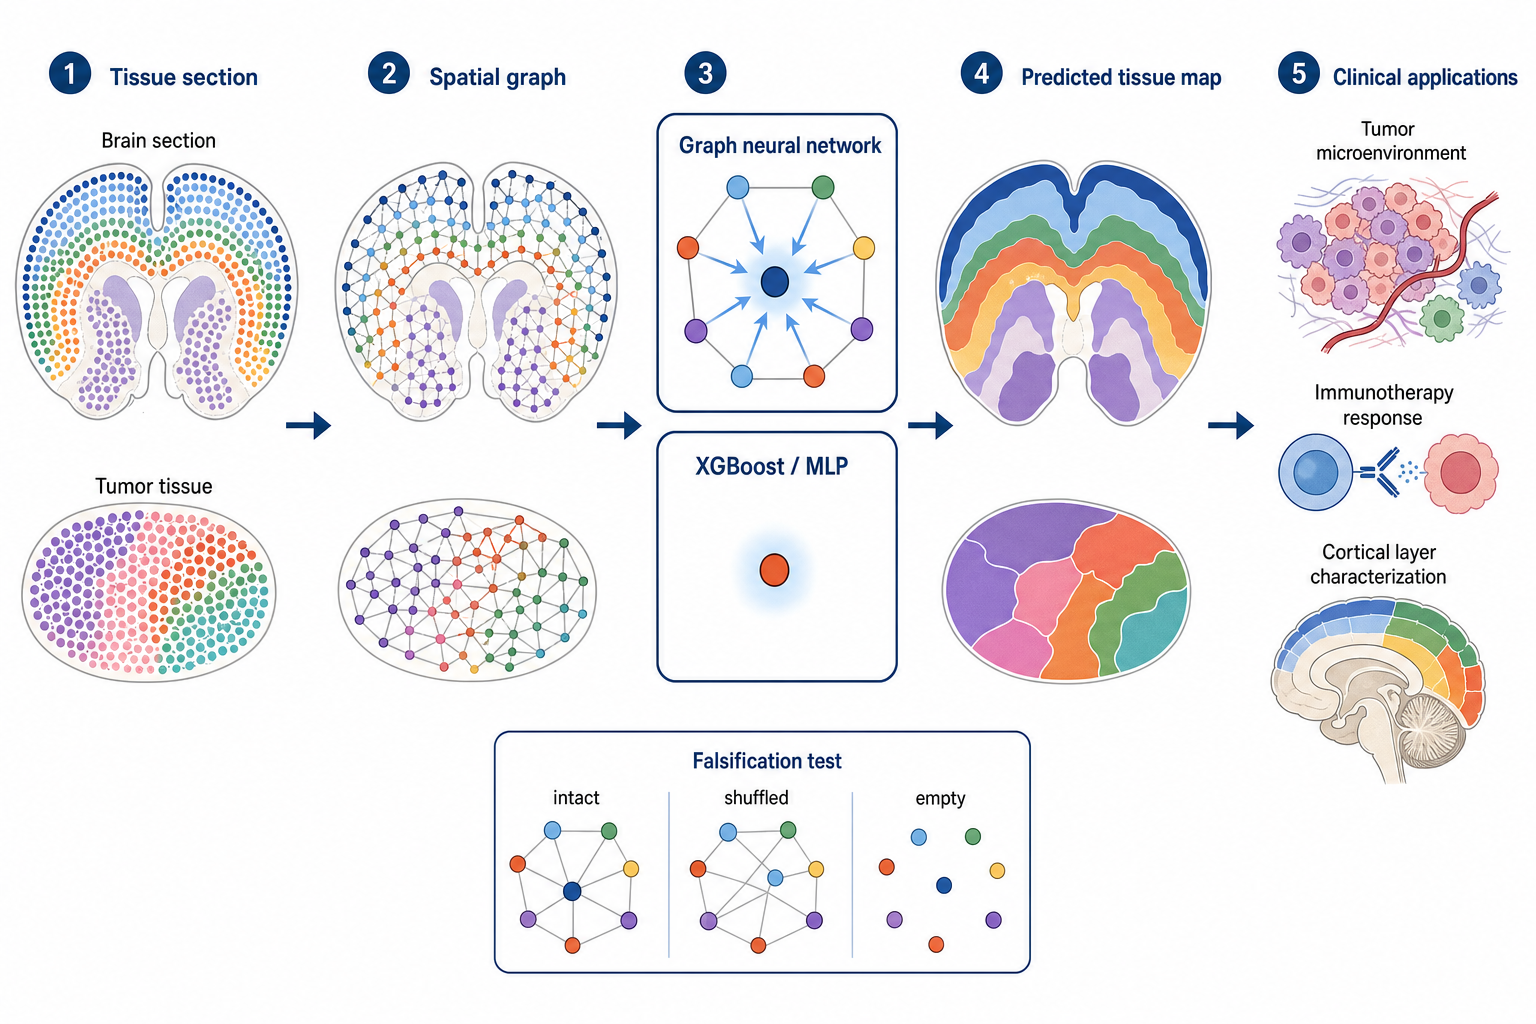
\includegraphics[width=\linewidth]{study_overview.png}
\caption{Study overview. Each spatial-transcriptomics section (human cortex or
tumor tissue) is turned into a graph whose nodes are spots or cells and whose
edges connect spatial neighbours. A graph neural network labels each spot by
pooling its neighbourhood, while XGBoost and MLP baselines see the same
expression features but treat each spot in isolation. We compare the predicted
tissue maps, run a falsification test that shuffles or removes the graph, and
connect the method to downstream uses in oncology and neuropathology.}
\label{fig:overview}
\end{figure}

% ===========================================================================
\section{Background and Significance}

\textbf{Why spatial context is clinically important.} Tissue function depends on
how cells are arranged in space. In the cerebral cortex, six layers (L1--L6)
above the white matter each carry distinct cell types and gene programs. In a
tumor, malignant cells, stroma, blood vessels, and infiltrating immune cells form
spatially structured niches. Disease changes are often spatially localized: tau
pathology in Alzheimer's follows a laminar gradient, schizophrenia shows
layer-specific cortical deficits, and a tumor's response to immunotherapy depends
on where immune cells sit relative to the malignant front. Standard bulk RNA
sequencing averages this away. Spatial transcriptomics (10x Visium, MERFISH,
Xenium, CosMx, Stereo-seq) preserves it, and a 2024 review in the Journal of
Cancer Research and Clinical Oncology argues that this spatial information can
advance precision oncology by capturing tumor heterogeneity, metastasis,
prognosis, and immunotherapy response that bulk profiling misses
\cite{cilento2024}.

\begin{table}[H]
\centering\small
\begin{tabular}{>{\raggedright\arraybackslash}p{0.30\linewidth} >{\raggedright\arraybackslash}p{0.62\linewidth}}
\toprule
\rowcolor{sriblue}\color{white}\textbf{Why it matters} & \color{white}\textbf{Consequence}\\
\midrule
\rowcolor{srirow} Tissue function is spatially organized & Disease changes are region/layer-specific, not diffuse.\\
Spatial omics preserves location & We can finally ask \emph{where} pathology starts.\\
\rowcolor{srirow} But spots must be assigned to a domain first & Domain mapping is an important early step for most downstream spatial analyses.\\
\bottomrule
\end{tabular}
\caption{Accurate spatial-domain mapping is the step that turns a
spatial-transcriptomics slide into interpretable, region-resolved biology, in
both brain disease and cancer.}
\label{tab:significance}
\end{table}

% ===========================================================================
\section{The Computational Gap}

Domain mapping is hard for two complementary reasons, and current practice
addresses neither well.

\begin{gapbox}
\textbf{Gap 1. Manual annotation does not scale.} Expert annotation of a single
section is slow and subjective. A disease cohort spans dozens of sections across
many donors, where hand-labelling becomes the bottleneck.\\[3pt]
\textbf{Gap 2. Per-spot expression is weak and structure-blind.} A single spot's
expression is sparse and dropout-corrupted, so models that classify each spot in
isolation (XGBoost, MLP) reach an accuracy ceiling and yield spatially fragmented
domains.
\end{gapbox}

\noindent The observation behind our approach is straightforward: a spot's domain
is largely a property of its spatial neighbourhood. Adjacent spots usually share
a domain, so the signal missing from one noisy spot is present in the tissue
around it (Fig.~\ref{fig:mechanism}). A model that can use the neighbourhood
should therefore do better than one that cannot, and the size of that gap is a
direct measure of how much the spatial structure is worth.

\begin{figure}[H]
\centering
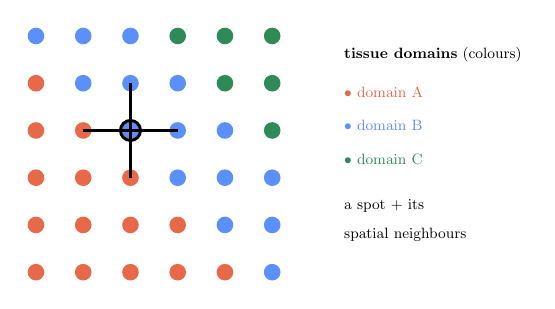
\begin{tikzpicture}[scale=0.6,every node/.style={transform shape}]
  \foreach \i in {0,...,5}{
    \foreach \j in {0,...,5}{
      \pgfmathtruncatemacro{\sum}{\i+\j}
      \ifnum\sum<5
        \definecolor{cc}{HTML}{E8684A}
      \else
        \ifnum\sum<8 \definecolor{cc}{HTML}{5B8FF9}\else\definecolor{cc}{HTML}{2E8B57}\fi
      \fi
      \node[circle,fill=cc,minimum size=10pt,inner sep=0pt] (n\i\j) at (\i,\j) {};
    }
  }
  \node[circle,draw=black,line width=1.1pt,minimum size=12pt,inner sep=0pt] at (2,3) {};
  \foreach \a/\b in {1/3,3/3,2/2,2/4}{\draw[black,line width=1pt] (2,3)--(\a,\b);}
  \node[anchor=west,font=\small] at (6.4,4.6) {\textbf{tissue domains} (colours)};
  \node[anchor=west,font=\small,domA] at (6.4,3.8) {$\bullet$ domain A};
  \node[anchor=west,font=\small,domB] at (6.4,3.1) {$\bullet$ domain B};
  \node[anchor=west,font=\small,domC] at (6.4,2.4) {$\bullet$ domain C};
  \node[anchor=west,font=\small] at (6.4,1.4) {a spot + its};
  \node[anchor=west,font=\small] at (6.4,0.8) {spatial neighbours};
\end{tikzpicture}
\caption{Domains are spatially contiguous, so a spot's label tends to agree with
its neighbours'. A single noisy spot may be ambiguous, but its neighbourhood
reveals its domain, which is the signal a spatial model can use and a per-spot
model cannot.}
\label{fig:mechanism}
\end{figure}

% ===========================================================================
\section{Central Hypothesis and Specific Aims}

\begin{problembox}
\textbf{Central hypothesis.} A spot's tissue domain is encoded not only in its
own gene expression but in its spatial neighbourhood. A graph neural network that
performs tissue-neighbour message passing should therefore map domains more
accurately than XGBoost and MLP models trained on the same expression features,
and removing the spatial graph should erase that advantage.
\end{problembox}

\begin{aimbox}{Specific Aims}
\textbf{Aim 1. Build and benchmark.} Develop a spatial GNN for tissue-domain
mapping and compare it directly against tuned XGBoost and an MLP on the same
features, under leakage-safe splits.\\
\textbf{Aim 2. Test whether the advantage is spatial.} Run a graph-removal test
(intact vs.\ shuffled vs.\ empty graph) on two tissues and technologies, and check
whether the GNN collapses to the MLP when the structure is destroyed.\\
\textbf{Aim 3. Ground it biologically and extend to cancer.} Recover known domain
marker genes, flag candidate annotation errors, and pilot the same pipeline on
tumor spatial transcriptomics to map microenvironment niches.
\end{aimbox}

% ===========================================================================
\section{Relationship to Prior Work}

GNN-based spatial-domain identification is an established field. SpaGCN
\cite{hu2021}, STAGATE \cite{dong2022}, and GraphST \cite{long2023} all apply
graph neural networks to spatial-omics data and are standard baselines on the
DLPFC benchmark.
We therefore do not claim a new architecture. Those methods are predominantly
unsupervised (graph autoencoders followed by clustering, scored by ARI against
manual labels) and are compared mainly against other clustering methods. Our
contribution is a complementary and, in this field, under-asked question: how
much does spatial structure actually add over strong non-graph models given the
same features? We answer it with (i) a supervised, leakage-safe cross-section
protocol (train on whole sections, predict held-out ones, which is the
disease-cohort regime); (ii) tuned XGBoost and MLP baselines on the same features,
which spatial-domain papers rarely report; (iii) a graph-removal test that
separates the spatial signal from model capacity; and (iv) replication across two
technologies (Visium and osmFISH). The deliverable is a careful
estimate of the value of tissue structure. It is a rigorous benchmark and
analysis, not a state-of-the-art or novel-method claim.

% ===========================================================================
\section{Datasets}

\begin{table}[H]
\centering\small
\begin{tabular}{>{\raggedright\arraybackslash}p{0.24\linewidth} >{\raggedright\arraybackslash}p{0.44\linewidth} >{\raggedright\arraybackslash}p{0.24\linewidth}}
\toprule
\rowcolor{sriblue}\color{white}\textbf{Dataset} & \color{white}\textbf{Content} & \color{white}\textbf{Role}\\
\midrule
\rowcolor{srirow} LIBD DLPFC (10x Visium) \cite{maynard2021,pardo2022} & 12 sections, 47{,}329 spots, expert manual layer labels (L1--L6 + WM) & Primary ground-truth benchmark (cross-section)\\
osmFISH mouse cortex \cite{codeluppi2018} & single-cell resolution, 33 genes, $\sim$4{,}839 cells, region labels & Second technology / generalization\\
\rowcolor{srirow} Controlled synthetic tissue & domains defined purely by neighbourhood; per-spot signal weak by construction & Mechanism isolation / sanity check\\
Tumor ST (Visium/Xenium, stretch) & public solid-tumor sections with niche annotations & Clinical extension (Aim 3)\\
\bottomrule
\end{tabular}
\caption{All data are public and de-identified. LIBD DLPFC is the field-standard
ground truth for spatial-domain methods. osmFISH tests a different assay with far
fewer genes, where per-cell features are weakest.}
\label{tab:data}
\end{table}

% ===========================================================================
\section{Methodology}

\textbf{From tissue to spatial graph.} Each section becomes a graph: nodes are
spots or cells, node features are preprocessed expression (normalize, log1p,
highly-variable genes, then PCA), and each node is connected to its $k$ nearest
spatial neighbours. The 2D coordinates are used only to build the graph, never as
model features, so any GNN benefit is attributable to message passing over tissue
structure rather than to memorizing absolute position.

\subsection{Model: a spatial graph neural network}
The GNN classifies each spot by pooling its neighbourhood over $L$ rounds of
message passing. With a GraphSAGE encoder,
\begin{equation}
h_v^{(l)} = \sigma\!\Big( W^{(l)}\big[\,h_v^{(l-1)} \,\big\Vert\,
\textstyle\operatorname*{AGG}_{u\in\NN(v)} h_u^{(l-1)}\,\big]\Big),
\qquad \hat{y}_v = \operatorname{softmax}\!\big(W_o\, h_v^{(L)}\big),
\label{eq:sage}
\end{equation}
trained with cross-entropy on annotated spots. Aggregation denoises the sparse
per-spot signal, which is the property Gap~2 lacks. We compare \textbf{GraphSAGE},
\textbf{GAT} (graph attention, which learns per-neighbour weights), and GCN
encoders; all use PyTorch Geometric.

\begin{figure}[H]
\centering
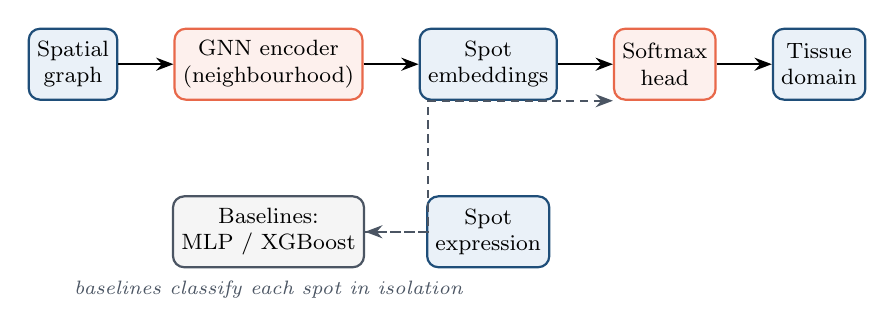
\begin{tikzpicture}[
  node distance=6mm and 7mm,
  box/.style={rounded corners,draw=sriblue,fill=srilight,thick,minimum height=0.9cm,align=center,font=\footnotesize,inner sep=3pt},
  red/.style={rounded corners,draw=sriaccent,fill=sriaccent!10,thick,minimum height=0.9cm,align=center,font=\footnotesize,inner sep=3pt},
  gray/.style={rounded corners,draw=srigray,fill=gray!8,thick,minimum height=0.9cm,align=center,font=\footnotesize,inner sep=3pt},
  >={Stealth[length=2.2mm]}]
  \node[box] (g) {Spatial\\graph};
  \node[red,right=of g] (enc) {GNN encoder\\(neighbourhood)};
  \node[box,right=of enc] (z) {Spot\\embeddings};
  \node[red,right=of z] (dec) {Softmax\\head};
  \node[box,right=of dec] (s) {Tissue\\domain};
  \draw[->,thick] (g)--(enc); \draw[->,thick] (enc)--(z);
  \draw[->,thick] (z)--(dec); \draw[->,thick] (dec)--(s);
  \node[gray,below=12mm of enc] (mlp) {Baselines:\\MLP / XGBoost};
  \node[box,below=12mm of z] (xf) {Spot\\expression};
  \draw[->,thick,densely dashed,srigray] (xf)--(mlp);
  \draw[->,thick,densely dashed,srigray] (mlp.east) -- ++(0.8,0) |- (dec.south west);
  \node[srigray,font=\scriptsize\itshape,below=1pt of mlp] {baselines classify each spot in isolation};
\end{tikzpicture}
\caption{Pipeline. The GNN (orange) pools each spot's spatial neighbourhood; the
non-spatial baselines (gray) classify each spot alone from the same features. The
only difference between them is access to the spatial graph.}
\label{fig:pipeline}
\end{figure}

\subsection{Baselines and leakage-safe evaluation}
We benchmark against tuned XGBoost and an MLP on the same expression features, so
the comparison isolates the value of tissue structure. We use three splits:
(i) \emph{cross-section}, where whole sections are held out for test (layer
layouts differ per section, so absolute position cannot transfer and only
neighbourhood-relative reasoning generalizes; this is the disease-cohort regime
and our headline test); (ii) \emph{within-section}, where contiguous spatial
blocks are held out; and (iii) \emph{stratified}, a standard transductive node
split for single-section data (osmFISH). In the cross-section disjoint-union
graph, train and test sections are separate connected components, so message
passing cannot leak labels across the split. We report accuracy, macro-F1
(domains are imbalanced), and the adjusted Rand index (ARI, the field-standard
domain metric), as mean $\pm$ std over seeds.

% ===========================================================================
\section{Preliminary Results}

A working pilot already supports the claims above.

\begin{table}[H]
\centering\small
\begin{tabular}{>{\raggedright\arraybackslash}p{0.30\linewidth} cccc}
\toprule
\rowcolor{sriblue}\color{white}\textbf{Macro-F1 / ARI} & \color{white}\textbf{XGBoost} & \color{white}\textbf{MLP} & \color{white}\textbf{SAGE} & \color{white}\textbf{GAT}\\
\midrule
\rowcolor{srirow} DLPFC, \emph{cross-section} (3 seeds) & 0.52 / 0.37 & 0.49 / 0.38 & \textbf{0.75 / 0.65} & \textbf{0.74 / 0.66}\\
osmFISH, \emph{within-section} (3 seeds) & 0.54 / 0.44 & 0.63 / 0.51 & \textbf{0.96 / 0.95} & \textbf{0.97 / 0.95}\\
\bottomrule
\end{tabular}
\caption{Spatial GNNs beat the non-spatial baselines on the same features, on two
tissues and two technologies. The osmFISH gap is larger because its 33-gene
per-cell signal is weakest, so the neighbourhood matters most. osmFISH is a single
section, so this is a transductive within-section split, an easier regime than
DLPFC's cross-section test, and is reported as such.}
\label{tab:prelim}
\end{table}

\begin{figure}[H]
\centering
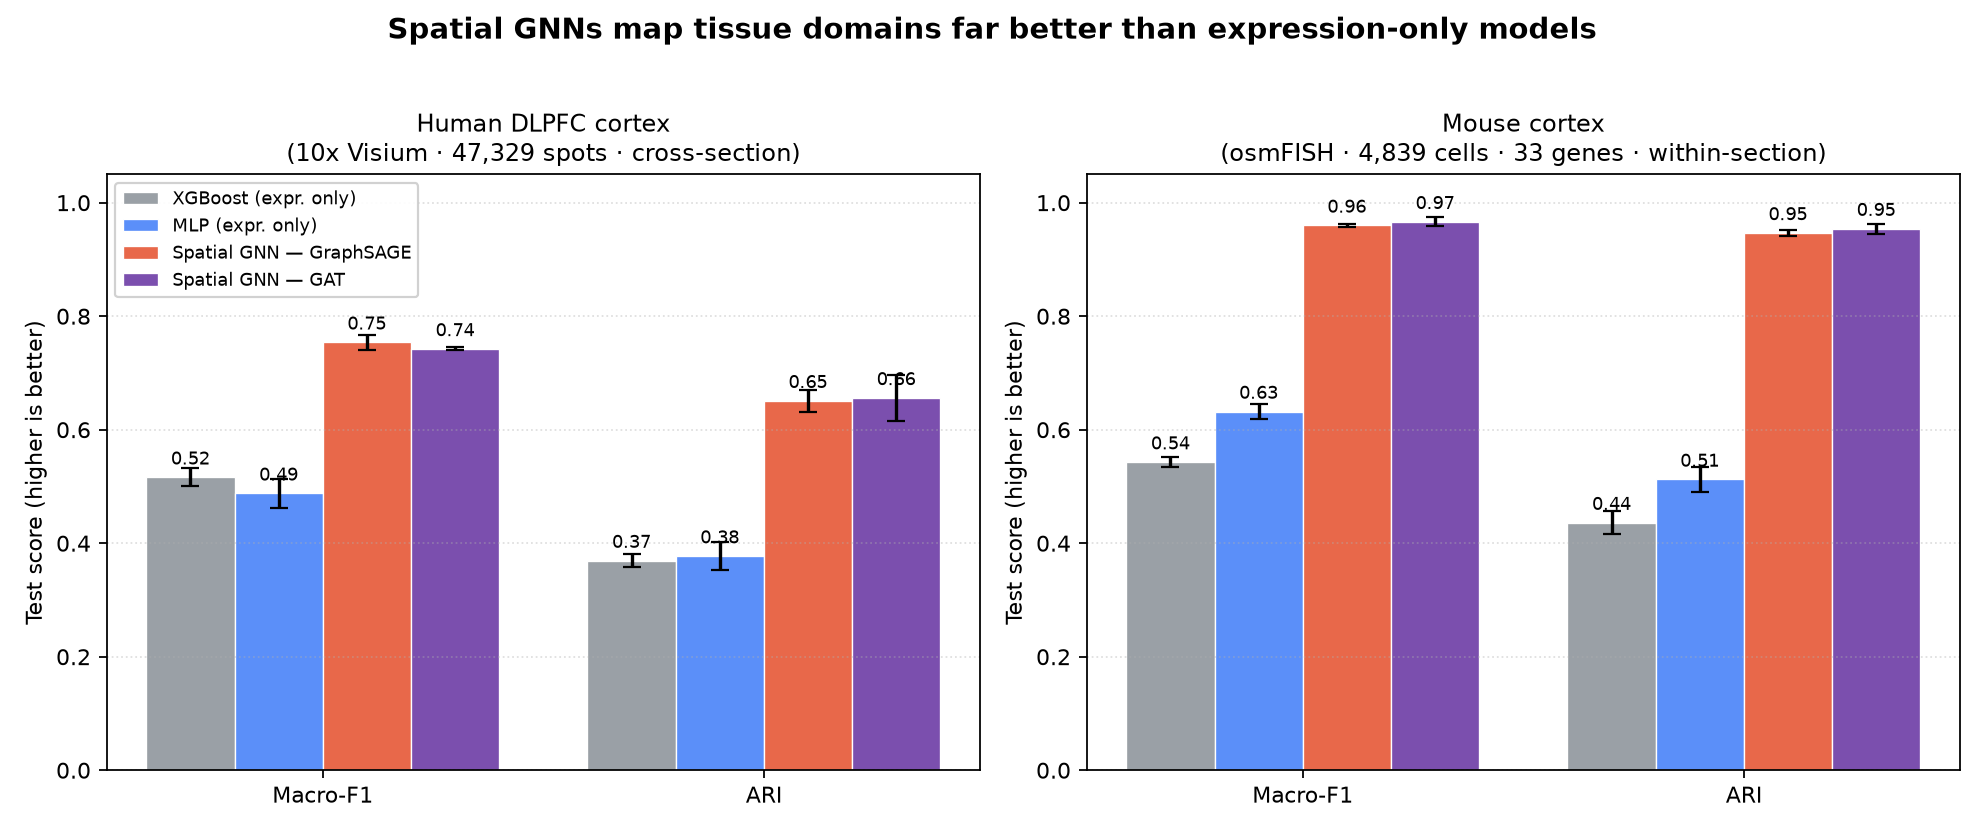
\includegraphics[width=\linewidth]{fig1_real_comparison.png}
\caption{Headline comparison. On both human DLPFC (Visium) and mouse cortex
(osmFISH), the spatial GNN (GraphSAGE and GAT) clearly outperforms XGBoost and
MLP, which see the same expression features but not the tissue graph.}
\label{fig:comparison}
\end{figure}

% ===========================================================================
\section{Rigor: Falsification and Biological Interpretation}

\subsection{Is the spatial structure really doing the work?}
We run the same GNN on three graphs. If the gain is genuinely spatial, destroying
the tissue structure should erase it, and it does, on both tissues
(Fig.~\ref{fig:ablation}, Table~\ref{tab:ablation}).

\begin{table}[H]
\centering\small
\begin{tabular}{>{\raggedright\arraybackslash}p{0.30\linewidth} cccc}
\toprule
\rowcolor{sriblue}\color{white}\textbf{GNN macro-F1} & \color{white}\textbf{Intact graph} & \color{white}\textbf{Shuffled edges} & \color{white}\textbf{Empty graph} & \color{white}\textbf{MLP ref.}\\
\midrule
\rowcolor{srirow} DLPFC (cross-section) & \textbf{0.75} & 0.49 & 0.49 & 0.48\\
osmFISH (within-section) & \textbf{0.95} & 0.58 & 0.61 & 0.63\\
\bottomrule
\end{tabular}
\caption{Falsification test. Replacing the true spatial $k$NN graph with
degree-matched random edges, or with no edges, collapses the GNN onto the blind
MLP on both tissues. The advantage comes from the graph, not the network
capacity.}
\label{tab:ablation}
\end{table}

\begin{figure}[H]
\centering
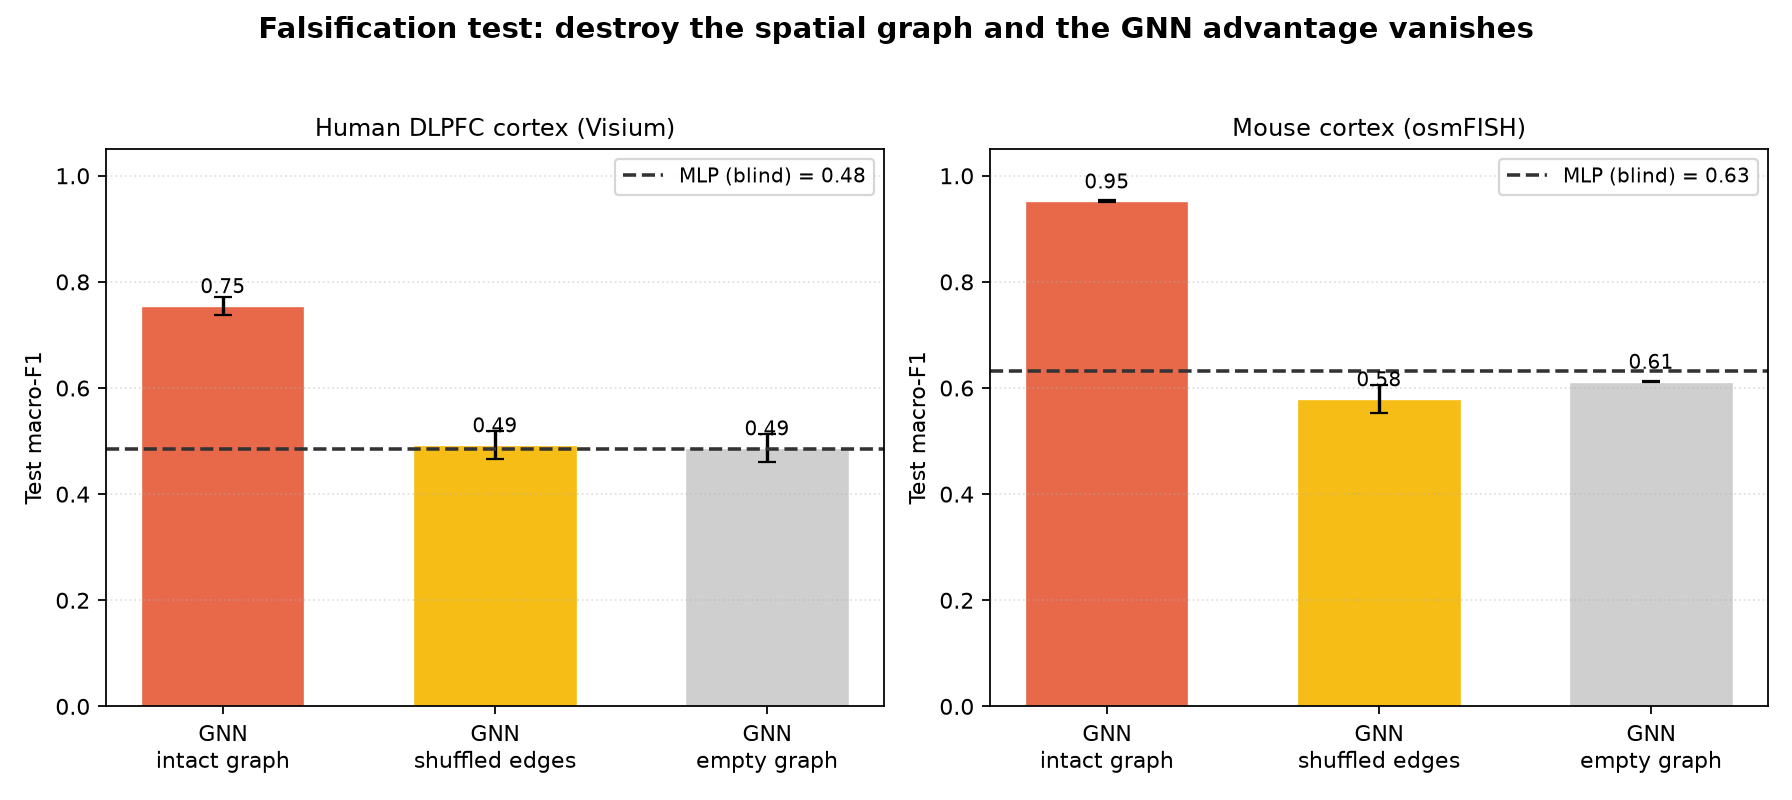
\includegraphics[width=\linewidth]{fig2_real_ablation.png}
\caption{The same falsification test, visualized on both tissues. Only the intact
spatial graph clears the MLP reference line; shuffled and empty graphs fall back
to it.}
\label{fig:ablation}
\end{figure}

\subsection{From accuracy to biology}
For each predicted domain we will (i) extract the genes driving predictions and
confirm recovery of known marker genes (cortical-layer markers for DLPFC), and
(ii) flag spots where the model confidently disagrees with the manual label,
which are candidate annotation errors or genuine micro-domains for expert review.
This turns an accuracy number into a hypothesis a biologist can act on.

% ===========================================================================
\section{Clinical Translation: Toward Precision Pathology}

The cortical-layer benchmark serves as the proof of concept. The same capability,
accurate and automated domain mapping that stays spatially coherent, is one
requirement for translating spatial transcriptomics to the clinic, particularly
in oncology \cite{cilento2024}.

\begin{table}[H]
\centering\small
\begin{tabular}{>{\raggedright\arraybackslash}p{0.30\linewidth} >{\raggedright\arraybackslash}p{0.62\linewidth}}
\toprule
\rowcolor{sriblue}\color{white}\textbf{Application} & \color{white}\textbf{How domain mapping helps}\\
\midrule
\rowcolor{srirow} Tumor microenvironment & Separate tumor core, invasive front, stroma, and immune niches to study heterogeneity and metastasis.\\
Immunotherapy response & Localize where immune cells sit relative to malignant cells, a spatial correlate of response.\\
\rowcolor{srirow} Neuro-/neurodegenerative disease & Pinpoint which cortical layers carry early molecular pathology (Alzheimer's, schizophrenia).\\
Pathologist support & Annotate complex molecular slides faster and more reproducibly than manual labelling.\\
\bottomrule
\end{tabular}
\caption{The brain benchmark tests the method; precision oncology and pathology
are where it pays off. All predictions are research-only and hypothesis-generating.}
\label{tab:clinical}
\end{table}

% ===========================================================================
\section{Project Strengths and Feasibility}

A few things give me confidence that the project is both feasible and worthwhile
(Table~\ref{tab:formula}): it uses real, public data; it has a clear medical
motivation; it compares against tuned non-graph baselines under leakage-safe
splits; it includes a causal check on where the gain comes from; and it ties the
accuracy back to known biology.

\begin{table}[H]
\centering\small
\begin{tabular}{>{\raggedright\arraybackslash}p{0.30\linewidth} >{\raggedright\arraybackslash}p{0.62\linewidth}}
\toprule
\rowcolor{sriblue}\color{white}\textbf{Criterion} & \color{white}\textbf{Commitment}\\
\midrule
\rowcolor{srirow} Real, sizable public data & LIBD DLPFC: 12 sections, 47k annotated spots, plus a second technology (osmFISH).\\
Clear medical motivation & Spatially-resolved localization of disease pathology; precision oncology bridge.\\
\rowcolor{srirow} Rigorous evaluation & Tuned XGBoost and MLP baselines; leakage-safe splits; multi-seed macro-F1 and ARI.\\
Causal / falsification test & Graph-removal ablation on two tissues collapses the GNN to the MLP.\\
\rowcolor{srirow} Interpretability $\rightarrow$ discovery & Recover marker genes; surface candidate annotation errors.\\
Transparent reporting & Any narrowing of the gap (e.g.\ easier transductive splits) is reported as-is.\\
\bottomrule
\end{tabular}
\caption{Strengths and feasibility of the project.}
\label{tab:formula}
\end{table}

% ===========================================================================
\section{Eight-Week Timeline}

The pilot already de-risks the core pipeline. The eight-week plan focuses on
validation, ablations, biological interpretation, and the tumor-ST extension
(Table~\ref{tab:timeline}).

\begin{table}[H]
\centering\small
\begin{tabular}{>{\raggedright\arraybackslash}p{0.14\linewidth} >{\raggedright\arraybackslash}p{0.78\linewidth}}
\toprule
\rowcolor{sriblue}\color{white}\textbf{Weeks} & \color{white}\textbf{Milestones}\\
\midrule
\rowcolor{srirow} 1--2 & Data pipeline (DLPFC + osmFISH to AnnData; spatial-graph builder); synthetic sanity check.\\
3--4 & Spatial GNN (SAGE/GAT/GCN) + tuned XGBoost + MLP; shared leakage-safe trainer.\\
\rowcolor{srirow} 5 & Cross-section, within-section, stratified experiments; multi-seed macro-F1/ARI.\\
6 & Falsification ablations (graph removal, depth, neighbourhood size) on both tissues.\\
\rowcolor{srirow} 7 & Biological interpretation (marker recovery, annotation-error flags); tumor-ST pilot.\\
8 & Figures, tables, manuscript draft; reproducibility package.\\
\bottomrule
\end{tabular}
\caption{Schedule for the eight-week SRI cohort. The pilot covers the core
pipeline, so the schedule focuses on validation, ablations, interpretation, and
the tumor-ST extension.}
\label{tab:timeline}
\end{table}

% ===========================================================================
\section{Reproducibility and Ethics}

Implementation uses open tools (PyTorch Geometric for the GNN; scanpy and anndata
for spatial-omics I/O; XGBoost). All code, configs, random seeds, and a data
manifest are released, and every reported number is multi-seed with standard
deviations. No human subjects are involved; all inputs are public, de-identified
post-mortem or model-organism tissue. Predictions are research-only and
hypothesis-generating and do not constitute clinical guidance.

% ===========================================================================
\begin{thebibliography}{9}
\small
\bibitem{cilento2024} Cilento MA, Sweeney CJ, Butler LM. \textit{Spatial
transcriptomics in cancer research and potential clinical impact: a narrative
review}. Journal of Cancer Research and Clinical Oncology, 150(6):296, 2024.
doi:10.1007/s00432-024-05816-0. PMID:~38850363.
\bibitem{maynard2021} Maynard KR, Collado-Torres L, et al. \textit{Transcriptome-
scale spatial gene expression in the human dorsolateral prefrontal cortex}.
Nature Neuroscience, 24:425--436, 2021.
\bibitem{pardo2022} Pardo B, et al. \textit{spatialLIBD: an R/Bioconductor package
to visualize spatially-resolved transcriptomics data}. BMC Genomics, 23:434, 2022.
\bibitem{codeluppi2018} Codeluppi S, et al. \textit{Spatial organization of the
somatosensory cortex revealed by osmFISH}. Nature Methods, 15:932--935, 2018.
\bibitem{long2023} Long Y, et al. \textit{Spatially informed clustering,
integration, and deconvolution of spatial transcriptomics with GraphST}. Nature
Communications, 14:1155, 2023.
\bibitem{dong2022} Dong K, Zhang S. \textit{Deciphering spatial domains from
spatially resolved transcriptomics with an adaptive graph attention auto-encoder
(STAGATE)}. Nature Communications, 13:1739, 2022.
\bibitem{hu2021} Hu J, et al. \textit{SpaGCN: integrating gene expression, spatial
location and histology to identify spatial domains using graph convolutional
networks}. Nature Methods, 18:1342--1351, 2021.
\bibitem{hamilton2017} Hamilton WL, Ying R, Leskovec J. \textit{Inductive
representation learning on large graphs (GraphSAGE)}. NeurIPS, 2017.
\bibitem{velickovic2018} Veli\v{c}kovi\'c P, et al. \textit{Graph Attention
Networks}. ICLR, 2018.
\end{thebibliography}

\end{document}
